\infolevone{
\subsection{Heavy Gas Cherenkov Detector}

A charged particle traveling faster
than the speed of light in the medium will create an electromagnetic
disturbance in the medium. The radiation emitted by this process is
called Cherenkov radiation after its discoverer.

Cherenkov radiation is conically distributed about the trajectory of the
particle, with an angle given by
$$
	\cos{\theta} = \frac{1}{\beta n}
$$
where the index of refraction $n = c/u$ and $\beta = v/c$, with $c$
the speed of light in vacuum, $u$ the speed of light in the medium,
and $v$ the speed of the particle.

The index of refraction allows one to control the threshold particle velocity
$v_{T}=u=c/n$ below which there is no Cherenkov light produced, and above which there
is Cherenkov light produced.  For a gas, the quantity $n-1$ is proportional to the pressure,
so adjusting the pressure of the gas allows one to select the
threshold velocity. Adjusting the threshold velocity then allows one to select particles of
different mass.  Given the same momentum, two particles of different mass
will have different velocity.  Therefore, a Cherenkov detector can be tuned,
for instance, to distinguish electrons from pions.



The SHMS Heavy Gas
Cherenkov detector consists of a large cylindrical tank,
with outer flange diameter of 1.88~m or 74~inch, and bolt to bolt length
of 1.3~m or 51.1 inch. The detector contains four mirrors which focus
light onto four 5 inch Hamamatsu R1584 photo multiplier tubes (PMTs),
as shown in Fig~\ref{fig:hgc}.


The main detector cylinder is made of a 0.5~inch thick T6061-T6
Aluminum sheet with radius of 1.725~m or 67.9~inch. Both circular ends
have been covered with 0.04~inch thick 2024-T4 Aluminum windows. These
windows were hydrostatically formed (and hence tested) at a pressure
of 45 PSI.In addition, the windows were hydrostatically tested at a
pressure of 60 PSI. The tank itself was helium leak checked and is
leak free on a scale of 10$^{-8}$ Atm-cm$^3$/s. HGC detector
configuration only allows sub atmospheric pressure operation, thus
under no circumstance the detector pressure shall exceed 1 Atm. Each
of the aluminum windows are sandwiched between the detector vessel and
a thick aluminum flange. All three components are clamped with
stainless steel bolts with washers and silicon bronze
nuts. Installation torque for each bolt is specified to be 26~lb$\cdot$ft.

%Detailed information on this testing program can be found in \cite {bi:tank}, \cite {bi:wind}.
%
% \subsection{PMT}
%
% PMT is not located inside of the vessel inclosure!
%
%
% PMT required negative voltage !
%
% Discharge
%
%

%	The HMS Cherenkov detector consists of a large cylindrical
%tank, $\phi_{in} = 59"$, $L = 60"$, containing two mirrors which focus
%light onto two 5 inch Burle 8854 multiplier photo  tubes (PMT's). The tank
%has been installed with 0.04 inch thick 2024-T3 Aluminum windows
%covering the circular ends of the cylindrical tank. These
%windows were hydrostatically formed (and hence tested) at a pressure
%of 28 PSI. The tank itself was helium leak checked and is leak free
%on a scale of 10$^{-8}$ Atm-cm$^3$/s. In addition, the tank was hydrostatically
%tested at a pressure of 35 PSI. Detailed information on this testing
%program can be found in \cite {bi:tank}, \cite {bi:wind}.


\begin{figure}[ht]
\centering
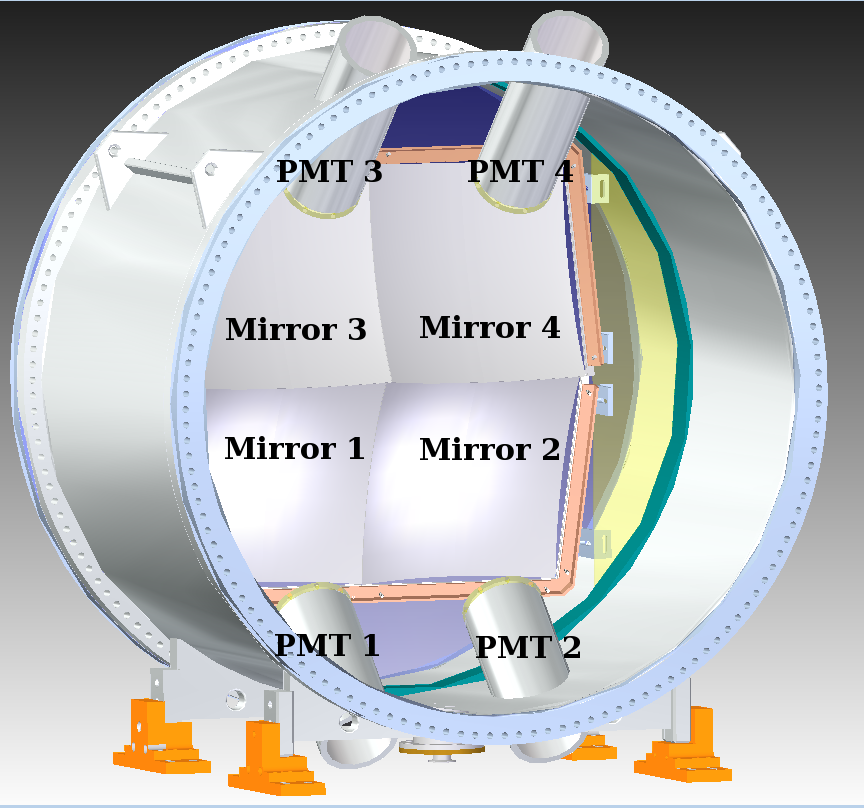
\includegraphics[width=0.75\linewidth]{cherenkov_front}
\caption{CAD Drawing of SHMS HGC detector. \label{fig:hgc}}
\end{figure}

The HGC tank is mounted on the detector rails using a three point alignment
scheme. The rails are easily capable of supporting the weight of the tank
without deformation. The gas handling system for the tank is designed to enable
the tank to be filled with gas suitable for the experiment.  Typically this 
would be C$_4$F$_8$O (C$_4$F$_{10}$), or CO2, at the desired operating pressure which is
0.2-1\,Atm. Detector operating pressure must not exceed 1 Atm.

The system consists of a dual-bottle gas manifold for the production gas and a
third single-bottle manifold for a purge gas (nitrogen or CO2).  The bottle
rack is at floor height welded to the SHMS detector carriage under the stairs
on the large angle side.

%FIXME BDS verify popoff sizing and locations
A diagram of the gas circuit is reproduced in Fig.~\ref{fig:hgc-gas-system}.
Each gas bottle has its own regulator, and all should be set to a nominal
40\,psig.  The ultimate gas pressure delivered to the gas panel in the SHMS hut
is limited to less than 14\,psig by a pressure regulator at the manifold output
set to 12--13\,psi and protected by a 14\,psi popoff valve.

\begin{figure}[ht]
\centering
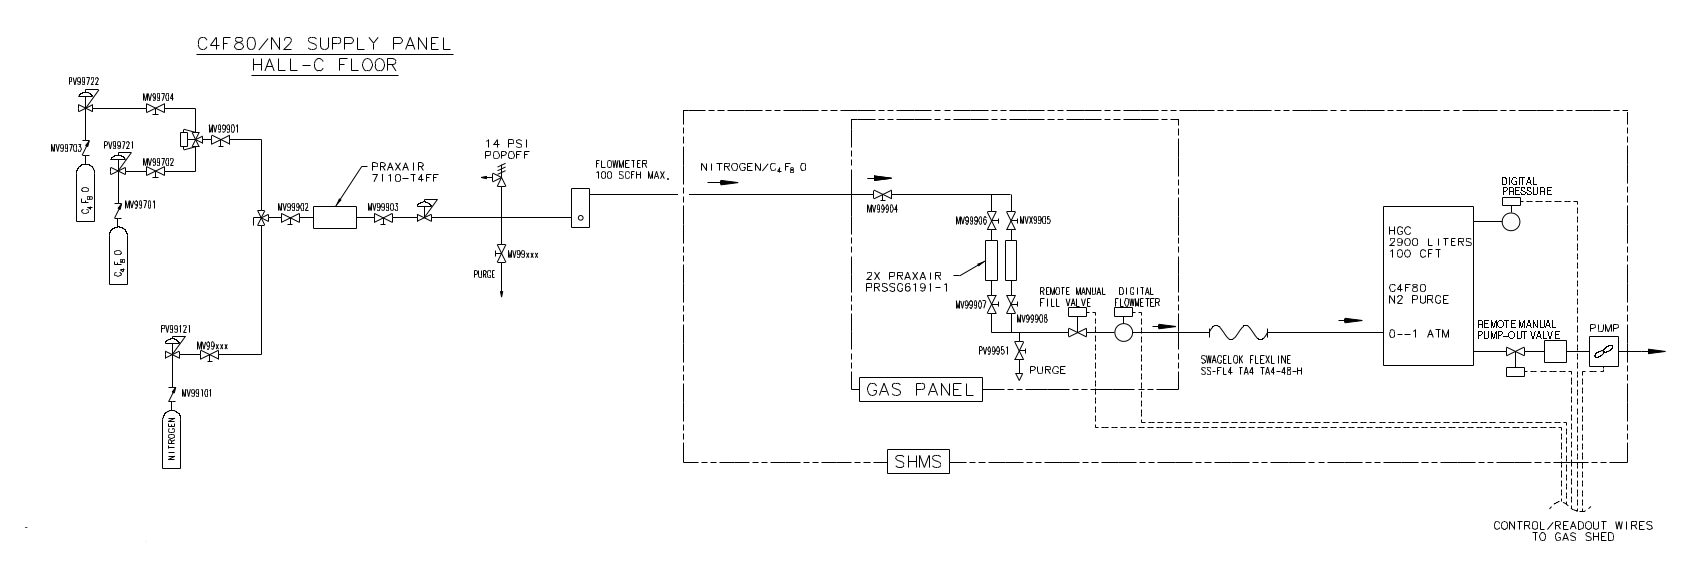
\includegraphics[width=\columnwidth]{hgc-gas-diagram.png}
\caption{CAD Drawing of SHMS HGC gas system (excerpt from JLab Drawing 67165-00100).}
\label{fig:hgc-gas-system}
\end{figure}

The gas flows through a 14X molecular sieve located on the SHMS detector gas
panel in the detector hut to hedge against contamination and is delivered to
the tank through a fill valve.  A digital flow-meter monitors and logs the gas
being delivered, and a digital pressure gauge records the pressure in the tank.
Communication between the digital pressure gauge and digital fill valve limits
the final pressure in the tank.  A 1\,psig popoff valve protects the tank from
unintended overpressure due to misconfiguration or equipment failure.

%FIXME BDS add pump model
Before filling, the tank is first cleaned by executing several pump and purge
cycles. The oil-free pump that used to evacuate the tank is located on a
platform welded directly beneath the HGC tank and can be controlled both
locally or remotely.  The fill valve is verified to be closed (it's normal
state), the pump engaged, and the pump-out valve opened.  Pressure in the tank
can be monitored both locally and remotely via the digital pressure gauge.

The mirrors in the HGC may require adjustment for optimal focusing on the PMT
faces. Small adjustment to the mirror position cannot be done while the
detector is mounted. The adjustment to mirror position can only be performed
when the detector vessel is in the horizontal position with both aluminum
windows completely removed. While the HGC is mounted, up to 1~cm adjustment to
PMT position can be made by repositioning the plastic eccentric PMT holders.
This adjustment should only be done by personnel who completely understand the
design of the PMT mounting assembly. 

%The interior of the tank has foot braces and welded hand holds which allow
%this work at the angle of the detector rails.

\paragraph{PMTs} From Fig~\ref{fig:hgc}, there are four aluminum sleeves welded onto
the detector cylinder, where each sleeve hosts one PMT assembly. Note
that the PMT assembly is outside of the vessel enclosure, viewing
the Cherenkov radiation through a quartz viewport. The inner end of
each sleeve is installed with a quartz window that provides vacuum
seal.  The rounded face of each Hamamatsu R1584 PMT is glued to a custom
flat-head quartz adapter. The PMT and quartz adapter is pressed
against the viewport, held in position via spring pressure. The
contacting optical surfaces are coupled with a thin layer of
UV-transparent silicon grease. A spring lock-in mechanism (open end of
the sleeve) is used to provide mechanical pressure to ensure good
contact between optical surfaces and a customized rubber cone is used
to provide a seal against light leaks.

% R1584 PMT assembly with a flat-head quartz adapter is pressed against the
% window, the contacting optical surfaces are coupled with a thin layer of UV
% transparent silicon grease;

\begin{table}[t]
\centering
  \begin{tabular}{ |c | c | c |}
    \hline
    PMT \#    & Serial \# & Voltage \\ \hline
    1         & LA0274    & 2132    \\ \hline
    2         & LA0272    & 1967    \\ \hline
    3         & LA0273    & 1926    \\ \hline
    4         & LA0271    & 2013    \\
    \hline
  \end{tabular}
  \caption{Serial number and initial recommended operating voltage for each PMT.} 
  \label{tab:hgc_volt}
\end{table}

The SHMS HGC 5~inch PMTs use {\bf negative} HV. The PMT photo-cathode
is powered using high negative voltage and the mu-metal shield
is grounded, so there is a ~2000\,V potential difference between the PMT
and the shield. Note that the Aerogel and Noble Gas Cherenkov
detectors use PMT bases that are designed for positive HV, therefore
one must only use labeled HV cables for HGC. The HV is supplied by
one pod of the {\em CAEN} power supply. The safe PMTs operating
voltages are between 1500 and 2400\,V. For the initial
commissioning stage, the operation voltages should not exceed 2200\,V.
The serial number and initial recommended operating voltages
for each PMT are listed in Table~\ref{tab:hgc_volt}. At the
recommended voltage, the expected average pulse height for a PMT
signal should be $\sim$400~mV and rates $\sim$100~Hz.

%at the time of installation we did extensive tests and confirmed no discharge.
%Then we can explain what might happen if there is a future breakdown of
%electrical insulation and what to look for.

Fig~\ref{hgc:goodsignal} shows an example of regular signal from a
R1584 PMT; Fig~\ref{hgc:discharge} shows an example of discharging
signal indicating a breach of electrical insulation between the
photo-cathode and mu-metal shield. The discharging signals have very
distinctive characteristics since they are relatively large pulses
($>$5 Volts) that are $>$100~ns long.

At the time of installation, extensive tests were performed for all
four PMTs and confirmed no discharge at 2000 Volts. Once discharging
signal is observed, one should carefully monitor the rate as well as
report the incidence immediately. The primary suspect for causing
discharge pulse is a possible electric insulation breach between the
photo tube and mu-metal shield. Further diagnose would require
complete removal of the PMT assembly from the aluminum sleeve while
all four PMTs are switched off. Electric insulation that covers the
inner edge of mu-metal shield cylinder must be carefully
inspected. Once the location of discharge is identified, it is
recommended to seal the suspect area with few layers kapton tape.


\begin{figure}
     \centering
     \subfloat[][Regular Signal]{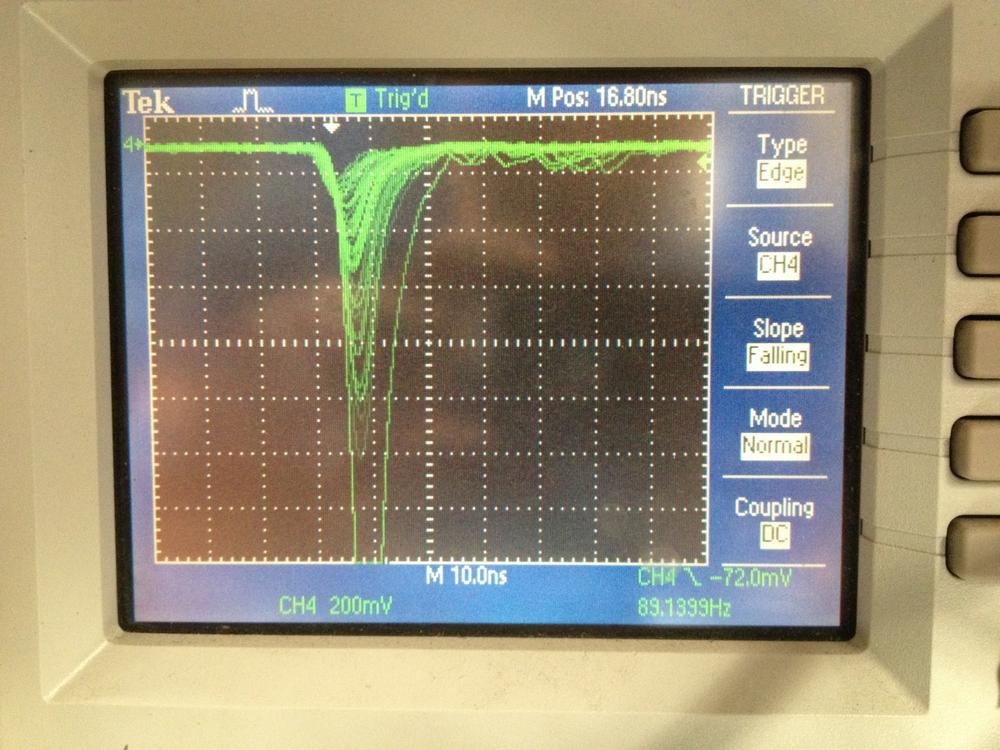
\includegraphics[width=0.45\linewidth]{pmt4_1047}\label{hgc:goodsignal}}~
     \subfloat[][Discharge]{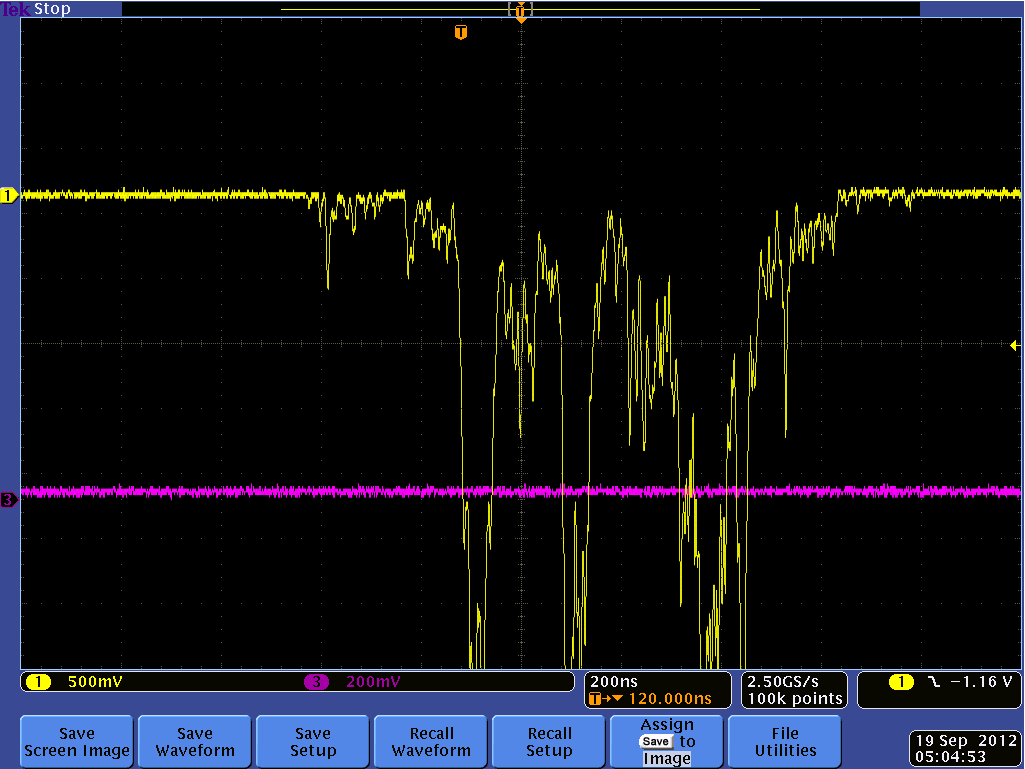
\includegraphics[width=0.45\linewidth]{discharge}\label{hgc:discharge}}
     \caption{(a) shows example of regular PMT signal; (b) shows a discharged signal.}
     \label{hgc:signal}
\end{figure}

%
% PMT serial number: LA0274, LA0272, LA0273, LA0271
%
% Initial recommanded voltage: 2132, 1967, 1926, 2013 Volts.
%

\paragraph{Operation Procedures}
%
The SHMS Heavy Gas Cherenkov Detector operates either as an $\pi$/$\kappa$ or
e/$\pi$ discriminator.  Figures~\ref{fig:c4f10-pressure-pi-kappa} and
\ref{fig:c4f10-pressure-e-pi} indicates suggested gas pressure vs. Cherenkov
threshold for various particles and SHMS momentum settings.  C$_4$F$_8$O and
C$_4$F$_{10}$ are functionally equivalent gases in this role.
See references~ \cite{docdb:SHMS-HGC-pi-kappa-docs} and \cite{docdb:SHMS-HGC-e-pi-docs}
for more detailed studies.

\begin{figure}
\centering
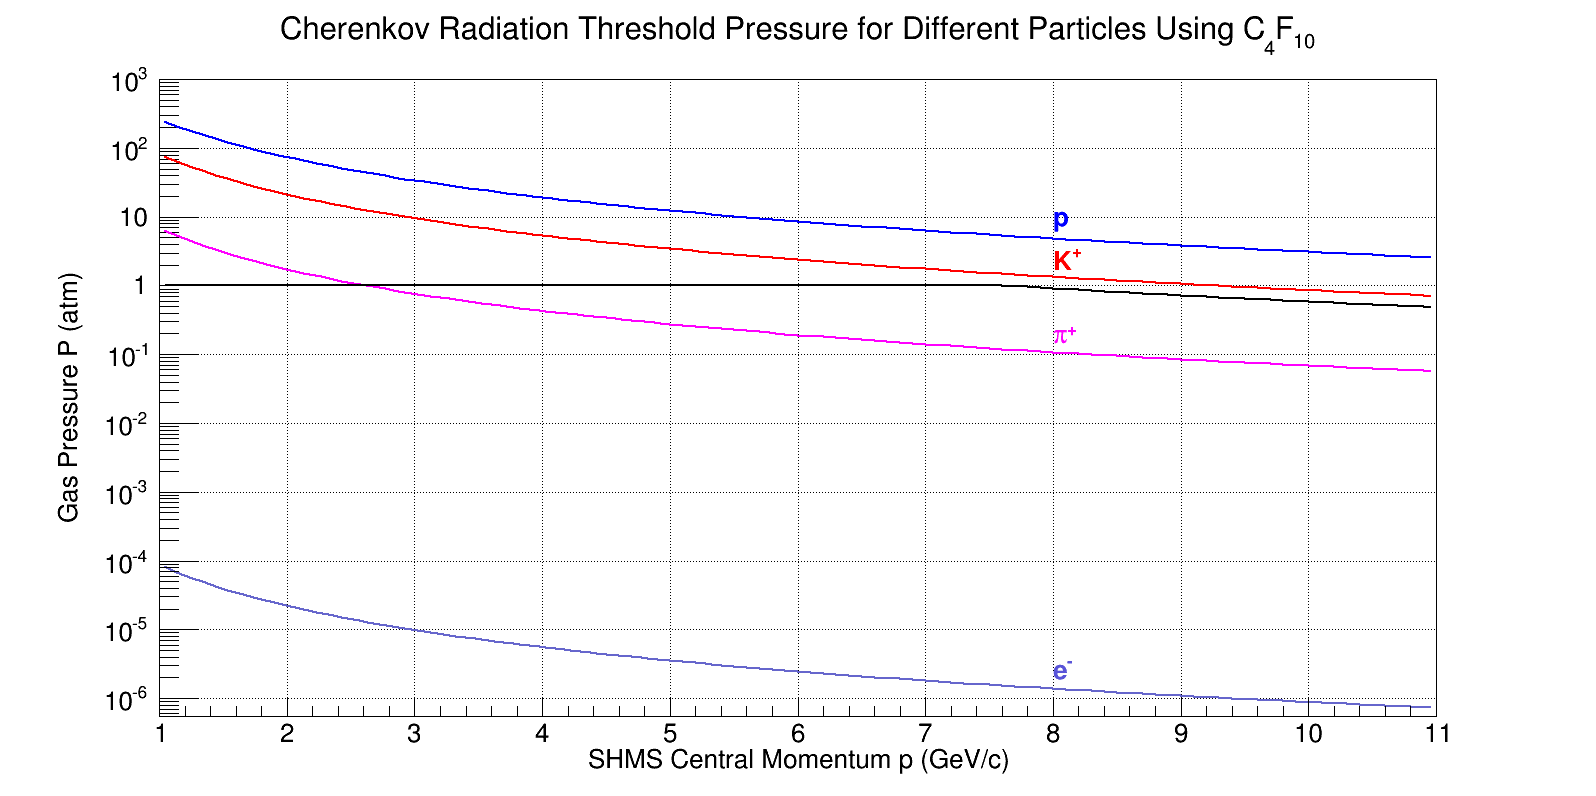
\includegraphics[width=\columnwidth]{c4f10_pressure-pi_kappa.png}
\caption{Gas Pressure vs. Particle Momentum. The black curve represents the
  suggested gas pressure of the HGC detector for good $\pi$/$\kappa$
  separation.  The colored curves represent the Cherenkov threshold pressure
  for different particles.  C$_4$F$_8$O performs equivalently to C$_4$F$_{10}$ in this
  context.
}
\label{fig:c4f10-pressure-pi-kappa}
\end{figure}

\begin{figure}
\centering
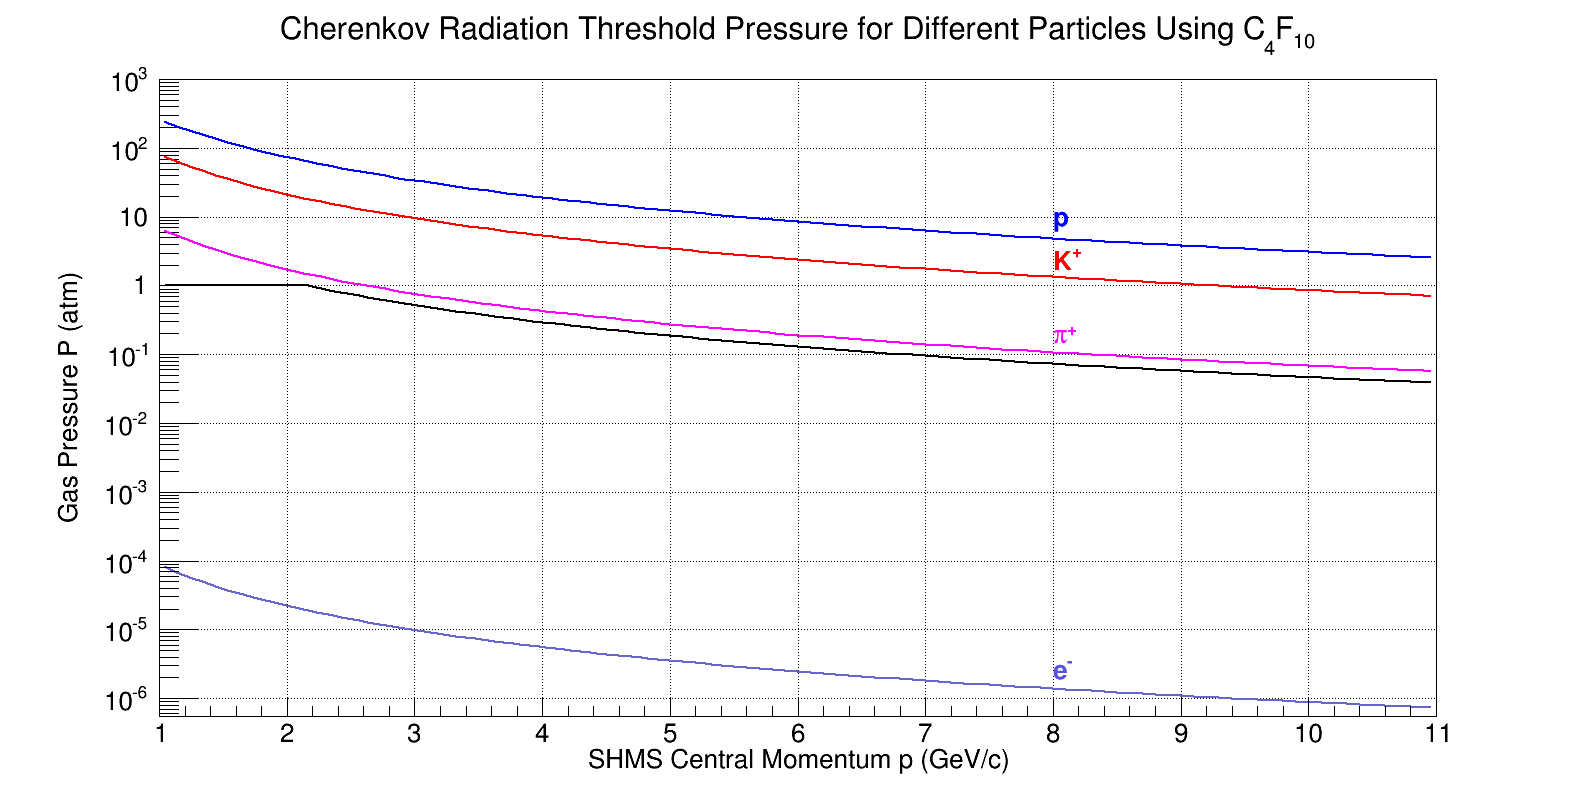
\includegraphics[width=\columnwidth]{c4f10_pressure-e_pi.png}
\caption{Gas Pressure vs. Particle Momentum. The black curve represents the
  suggested gas pressure of the HGC detector for good $e$/$\pi$
  separation. The colored curves represent the Cherenkov threshold pressure
  for different particles.  C$_4$F$_8$O performs equivalently to C$_4$F$_{10}$ in this context.
}
\label{fig:c4f10-pressure-e-pi}
\end{figure}

The nomenclature used in the description of these operation procedures refers
to the gas system diagram in Figure~\ref{fig:hgc-gas-system}.

\paragraph{$\bf{\pi}$/$\kappa$ Procedures}
This mode of operation typically requires the tank to be filled with C$_4$F$_8$O
(C$_4$F$_{10}$) at pressures varying from 0.2 to 1~Atm (absolute). The detector
is pumped down to ~1 millitorr, then refilled with C$_4$F$_8$O (C$_4$F$_{10}$)
gas.

Because the operating pressure is slightly subatmospheric, a pump and fill
procedure is employed.

%FIXME BDS (Add valve names, verify steps in detector hut)
\begin{enumerate}
  \item Initial Prep
  \begin{enumerate}
    \item Ensure that the HGC Remote Fill Valve is CLOSED.
    \item If you will changing the radiator gas, then ensure Valve
      \textbf{MV9902} is also CLOSED.  This is the main cut-off valve
      downstream of the 3-way valve on the supply gas panel under the stairs on
      the SHMS carriage.\label{hgc:step:changegas}
    \item Rotate the 3-way valve to connect the radiator gas you require to the
      downstream system.
    \item Leave the cut-off valve closed for now.
  \end{enumerate}

  \item The tank is now ready to be evacuated.
  \begin{enumerate}
    \item Turn ON the pump.  (This pump is oil-free and does not require a trap.)
    \item Very \emph{slowly} open the HGC Remote Pump-out Valve.  Since this
      valve connects the pump line to the detector volume, the pump will work
      hard.  Meter this valve so that the pump is never under extreme stress.  It
      will take approximately 20~minutes to pump down the tank.
      %FIXME BDS (may need to update this number after procedure is tested)
    \item Monitor the HGC Digital Pressure readback and close the HGC Remote
      Pump-out Valve when you have reached $\approx 1 10^{-3}$ Torr.
      %FIXME BDS (may need to update this number after procedure is tested)
    \item CLOSE the HGC Remote Pump-out Valve.
    \item Turn OFF the pump.
    \item Monitor the HGC Digital Pressure readback for a few moments and ensure
      it is stable!
  \end{enumerate}

  \item The tank can now be filled.
  \begin{enumerate}
    \item If required due to Step~\ref{hgc:step:changegas}, \emph{slowly} open
      the cut-off valve on the gas supply manifold under the SHMS stairs.
      Monitor the flow-meter on the same panel and ensure that you do
      \textbf{NOT} see any flow beyond that needed to pressurize the lines to
      the distribution panel in the SHMS detector hut.
    \item Slowly open the HGC Remote Fill Valve and monitor the Digital Flowmeter
      \emph{and} Digital pressure readbacks.  A reasonable flow is 20~cfpm.
    \item Monitor the HGC Digital Pressure readback and close the HGC Remote
      Fill Valve when you have reached the desired operating pressure.
    \item CLOSE the HGC Remote Fill Valve.
    \item If the tank will remain at this pressure for an extended period
      (\emph{i.e.} over a week, then CLOSE the main cutoff valve at the supply
      panel under the SHMS carriage stairs (\textbf{MV9902}).
  \end{enumerate}
\end{enumerate}

The fill should take approximately 30 minutes.  The detector should NEVER be
left unattended during a fill.  Frequently check the pressure in the tank and
be aware when the pressure is near to one atmosphere.  \textbf{DO NOT let the
  pressure exceed one atmosphere under any circumstances; doing so risks damage
to all of the equipment and personnel in the detector hut.}

% \paragraph{$e$/$\bf{\pi}$ Procedures}
% The procedure for $e$/$\bf{\pi}$ separation runs with 0.2 to
% 1 atmospheres of C$_4$F$_{10}$.  This is just a small modification to the
% current $\pi$/$\kappa$ procedures.

% $e$/$\bf{\pi}$ running can also be accomplished using a Nitrogen fill.
% This mode of operation requires the tank to be filled with approximately
% 13.5~psia of $\rm{N_2}$. The boiloff from the spectrometer magnets is a
% perfect source of clean, dry Nitrogen, and is normally used to fill the
% Cherenkov tank.


}%\infolevone{
